\ifdefined\included
\else
\documentclass[english,a4paper,11pt,twoside]{StyleThese}
\usepackage{amsmath,amssymb}             % AMS Math
\usepackage[T1]{fontenc}
\usepackage[utf8x]{inputenc}
\usepackage{babel}
\usepackage{datetime}

\usepackage{lmodern}
\usepackage{tabularx}
%\usepackage{tabular}
\usepackage{multirow}

\usepackage{subfigure}
\usepackage{fancyvrb}
\usepackage{algorithmic}
\usepackage{algorithm}
\usepackage{mathtools}


\usepackage{hhline}
\usepackage[left=1.5in,right=1.3in,top=1.1in,bottom=1.1in,includefoot,includehead,headheight=13.6pt]{geometry}
\renewcommand{\baselinestretch}{1.05}

% Table of contents for each chapter

\usepackage[nottoc, notlof, notlot]{tocbibind}
\usepackage{minitoc}
\setcounter{minitocdepth}{2}
\mtcindent=15pt
% Use \minitoc where to put a table of contents

\usepackage{aecompl}


% Glossary / list of abbreviations

\usepackage[intoc]{nomencl}
\iftoggle{ThesisInEnglish}{%
\renewcommand{\nomname}{Glossary}
}{ %
\renewcommand{\nomname}{Liste des Abréviations}
}

\newcommand{\accom}[1]{\textcolor{red}{[#1]}}

\makenomenclature

% My pdf code

\usepackage{ifpdf}

\ifpdf
  \usepackage[pdftex]{graphicx}
  \DeclareGraphicsExtensions{.jpg}
  \usepackage[a4paper,pagebackref,hyperindex=true]{hyperref}
  \usepackage{tikz}
  \usetikzlibrary{arrows,shapes,calc}
\else
  \usepackage{graphicx}
  \DeclareGraphicsExtensions{.ps,.eps}
  \usepackage[a4paper,dvipdfm,pagebackref,hyperindex=true]{hyperref}
\fi

\graphicspath{{.}{images/}}

%% nicer backref links. NOTE: The flag ThesisInEnglish is used to define the
% language in the back references. Read more about it in These.tex

\iftoggle{ThesisInEnglish}{%
\renewcommand*{\backref}[1]{}
\renewcommand*{\backrefalt}[4]{%
\ifcase #1 %
(Not cited.)%
\or
(Cited in page~#2.)%
\else
(Cited in pages~#2.)%
\fi}
\renewcommand*{\backrefsep}{, }
\renewcommand*{\backreftwosep}{ and~}
\renewcommand*{\backreflastsep}{ and~}
}{%
\renewcommand*{\backref}[1]{}
\renewcommand*{\backrefalt}[4]{%
\ifcase #1 %
(Non cité.)%
\or
(Cité en page~#2.)%
\else
(Cité en pages~#2.)%
\fi}
\renewcommand*{\backrefsep}{, }
\renewcommand*{\backreftwosep}{ et~}
\renewcommand*{\backreflastsep}{ et~}
}

% Links in pdf
\usepackage{color}
\definecolor{linkcol}{rgb}{0,0,0.4} 
\definecolor{citecol}{rgb}{0.5,0,0} 
\definecolor{linkcol}{rgb}{0,0,0} 
\definecolor{citecol}{rgb}{0,0,0}
% Change this to change the informations included in the pdf file

\hypersetup
{
bookmarksopen=true,
pdftitle="Joint Action for Human-Robot Interaction",
pdfauthor="Sandra DEVIN", %auteur du document
pdfsubject="Thesis", %sujet du document
%pdftoolbar=false, %barre d'outils non visible
pdfmenubar=true, %barre de menu visible
pdfhighlight=/O, %effet d'un clic sur un lien hypertexte
colorlinks=true, %couleurs sur les liens hypertextes
pdfpagemode=None, %aucun mode de page
pdfpagelayout=SinglePage, %ouverture en simple page
pdffitwindow=true, %pages ouvertes entierement dans toute la fenetre
linkcolor=linkcol, %couleur des liens hypertextes internes
citecolor=citecol, %couleur des liens pour les citations
urlcolor=linkcol %couleur des liens pour les url
}

% definitions.
% -------------------

\setcounter{secnumdepth}{3}
\setcounter{tocdepth}{2}

% Some useful commands and shortcut for maths:  partial derivative and stuff

\newcommand{\pd}[2]{\frac{\partial #1}{\partial #2}}
\def\abs{\operatorname{abs}}
\def\argmax{\operatornamewithlimits{arg\,max}}
\def\argmin{\operatornamewithlimits{arg\,min}}
\def\diag{\operatorname{Diag}}
\newcommand{\eqRef}[1]{(\ref{#1})}

\usepackage{rotating}                    % Sideways of figures & tables
%\usepackage{bibunits}
%\usepackage[sectionbib]{chapterbib}          % Cross-reference package (Natural BiB)
%\usepackage{natbib}                  % Put References at the end of each chapter
                                         % Do not put 'sectionbib' option here.
                                         % Sectionbib option in 'natbib' will do.
\usepackage{fancyhdr}                    % Fancy Header and Footer

% \usepackage{txfonts}                     % Public Times New Roman text & math font
  
%%% Fancy Header %%%%%%%%%%%%%%%%%%%%%%%%%%%%%%%%%%%%%%%%%%%%%%%%%%%%%%%%%%%%%%%%%%
% Fancy Header Style Options

\pagestyle{fancy}                       % Sets fancy header and footer
\fancyfoot{}                            % Delete current footer settings

%\renewcommand{\chaptermark}[1]{         % Lower Case Chapter marker style
%  \markboth{\chaptername\ \thechapter.\ #1}}{}} %

%\renewcommand{\sectionmark}[1]{         % Lower case Section marker style
%  \markright{\thesection.\ #1}}         %

\fancyhead[LE,RO]{\bfseries\thepage}    % Page number (boldface) in left on even
% pages and right on odd pages
\fancyhead[RE]{\bfseries\nouppercase{\leftmark}}      % Chapter in the right on even pages
\fancyhead[LO]{\bfseries\nouppercase{\rightmark}}     % Section in the left on odd pages

\let\headruleORIG\headrule
\renewcommand{\headrule}{\color{black} \headruleORIG}
\renewcommand{\headrulewidth}{1.0pt}
\usepackage{colortbl}
\arrayrulecolor{black}

\fancypagestyle{plain}{
  \fancyhead{}
  \fancyfoot{}
  \renewcommand{\headrulewidth}{0pt}
}

%\usepackage{MyAlgorithm}
%\usepackage[noend]{MyAlgorithmic}
\usepackage[ED=MITT - STICIA, Ets=INP]{tlsflyleaf}
%%% Clear Header %%%%%%%%%%%%%%%%%%%%%%%%%%%%%%%%%%%%%%%%%%%%%%%%%%%%%%%%%%%%%%%%%%
% Clear Header Style on the Last Empty Odd pages
\makeatletter

\def\cleardoublepage{\clearpage\if@twoside \ifodd\c@page\else%
  \hbox{}%
  \thispagestyle{empty}%              % Empty header styles
  \newpage%
  \if@twocolumn\hbox{}\newpage\fi\fi\fi}

\makeatother
 
%%%%%%%%%%%%%%%%%%%%%%%%%%%%%%%%%%%%%%%%%%%%%%%%%%%%%%%%%%%%%%%%%%%%%%%%%%%%%%% 
% Prints your review date and 'Draft Version' (From Josullvn, CS, CMU)
\newcommand{\reviewtimetoday}[2]{\special{!userdict begin
    /bop-hook{gsave 20 710 translate 45 rotate 0.8 setgray
      /Times-Roman findfont 12 scalefont setfont 0 0   moveto (#1) show
      0 -12 moveto (#2) show grestore}def end}}
% You can turn on or off this option.
% \reviewtimetoday{\today}{Draft Version}
%%%%%%%%%%%%%%%%%%%%%%%%%%%%%%%%%%%%%%%%%%%%%%%%%%%%%%%%%%%%%%%%%%%%%%%%%%%%%%% 

\newenvironment{maxime}[1]
{
\vspace*{0cm}
\hfill
\begin{minipage}{0.5\textwidth}%
%\rule[0.5ex]{\textwidth}{0.1mm}\\%
\hrulefill $\:$ {\bf #1}\\
%\vspace*{-0.25cm}
\it 
}%
{%

\hrulefill
\vspace*{0.5cm}%
\end{minipage}
}

\let\minitocORIG\minitoc
\renewcommand{\minitoc}{\minitocORIG \vspace{1.5em}}

\usepackage{multirow}
%\usepackage{slashbox}

\newenvironment{bulletList}%
{ \begin{list}%
	{$\bullet$}%
	{\setlength{\labelwidth}{25pt}%
	 \setlength{\leftmargin}{30pt}%
	 \setlength{\itemsep}{\parsep}}}%
{ \end{list} }

\newtheorem{definition}{Définition}
\renewcommand{\epsilon}{\varepsilon}

% centered page environment

\newenvironment{vcenterpage}
{\newpage\vspace*{\fill}\thispagestyle{empty}\renewcommand{\headrulewidth}{0pt}}
{\vspace*{\fill}}

\usepackage{tablefootnote}

\sloppy
\begin{document}
\dominitoc
\faketableofcontents
\fi


\chapter*{Introduction}
\addstarredchapter{Introduction} %Sinon cela n'apparait pas dans la table des matières
\minitoc

\section*{Context}
\addcontentsline{toc}{section}{Context}

In the 1940s, researchers invented the first machines that we can call computers. Then, they quickly came to think that this new tool which can easily manipulate numbers can also manipulate symbols and they started to work on new "thinking machines". In 1956, at the Dartmouth conference, the domain of "Artificial Intelligence" is recognized as a fully academic field. Associated to the automaton technology, the first "robots" quickly arrived in our environment.

Some of these robots are meant to work alone (e.g. rovers for space exploration) while others need to work in the vicinity and/or with humans. One possible example is robot "co-workers". These robots need to collaborate in a safe, efficient and fluent way with humans to accomplish more or less repetitive tasks. The last decades also witnessed the apparition of what is called "sociable robots" \cite{dautenhahn2007socially}. These robots can be used, for example, to help elderly or injured people in their daily life our to guide people in public spaces. 

The aim of this thesis is to make a step toward robots which act jointly with humans in a natural, efficient and fluent way. We focus more especially on the decisional issues that can appear during human-robot Joint Action. The subject of Joint Action between humans has been studied a lot in social sciences, however, many things remain to be discovered. Based on these results, the aim here is to build robots which are able to understand the humans (their beliefs and choices) and to adapt to them in order to be more pleasant and efficient companions.

\newpage
\section*{Human-Robot Joint Action challenges}
\addcontentsline{toc}{section}{Human-Robot Joint Action challenges}

Constructing robots which are able to smoothly execute Joint Action with humans brings a number of challenges. 

A first prerequisite for the robot is to be engaged in the Joint Action. If the goal is not imposed by its human partner, the robot needs to pro-actively propose its help whenever it is needed. Then, the robot needs to monitor its partner engagement in the task and demonstrate its engagement in the same task.

Once the robot has a goal to achieve, it needs to be able to find a plan to achieve this goal. This plan should be feasible in the current context of course, but it should also take the human into account, his abilities and preferences. Once a plan found, the robot should be able to share it or negotiate it with its partner. Only then, the execution of the task can begin.

During the Joint Action execution, one first challenge for the robot is to be able to understand how the humans perceive their environment and what are their knowledge concerning the task. In other words, it needs to be able to constantly estimate the mental states of its partners. These mental states should be taken into account at every steps of the execution in order to unsure a good understanding between partners.

Finally, the robot needs to be able to coordinate with the human. This coordination is needed at all level of the execution. At a lower level, the robot should exhibit an understandable and predictable behavior when performing actions. It also needs to be able to execute actions such as handover which require precise motor coordination. At a higher level, the robot needs to coordinate the Shared Plan execution. It not only needs to execute its actions at the right time but it should also give the appropriate information at the right time to its partners using either verbal or non-verbal communication.

\section*{Contributions and manuscript organization}
\addcontentsline{toc}{section}{Contributions and manuscript organization}

At the beginning of the thesis, I add to main starting points. One of these points was, as in almost all thesis I guess, the current states of the art both in robotics and in social sciences concerning human-human Joint Action. The second starting point was the current architecture for human-robot interaction developed in my research group and more especially the supervision part which I was asked to work on it. The aim with all of this being to bring innovating changes to the current system (again as in most thesis I guess). The process which I followed during this thesis and which I will explain now is graphically resumed in Fig.~\ref{fig:planIntro}.

As a first step, I studied the bibliography concerning Joint Action between humans in order to better understand what are the needed components of a successful Joint Action. I also studied the current state of the art in robotics, and more especially in human-robot interaction, in order to have an overview of what robots was already capable of. Based on all of this, I identified the needed components of a successful Human-Robot Joint Action and I studied, always based on bibliography, how to articulate them into a coherent architecture. This part constitute the Chapter~\ref{ch:biblio} of the manuscript.

Then, I took a look at the current state of the architecture for human-robot interaction developed in my research group. I especially focused on the supervision part of the architecture which I was in charge to develop. Based on the conclusion of my bibliographic study, I was able to identify several possible improvements to bring to the supervisor. The final version of the supervisor in presented in Chapter~\ref{ch:Sup} in order to help the understanding of the following of the manuscript and constitute the major technical contribution of the thesis.

\begin{figure}[!t]
	\centering
    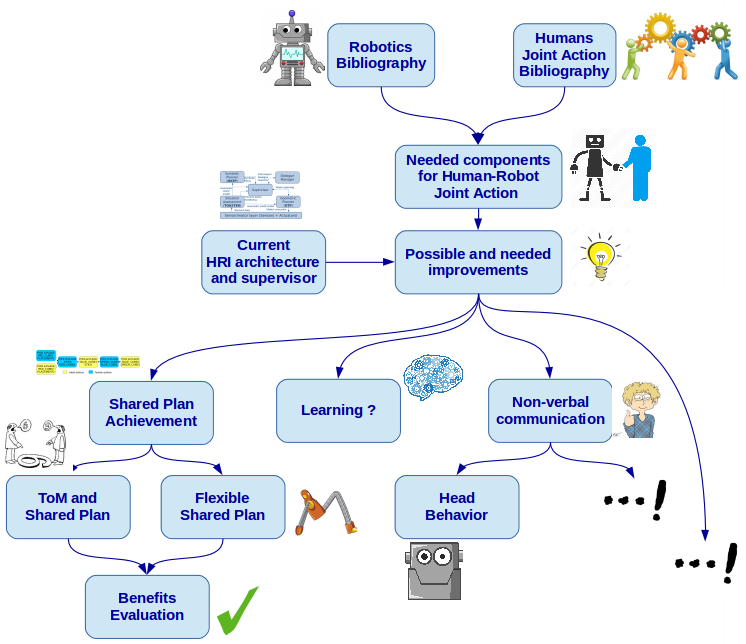
\includegraphics[width=\textwidth]{figs/Introduction/Plan.png}
    \caption{Organization of the contributions presented in the manuscript.}
    \label{fig:planIntro}
\end{figure}

One first subject where I saw possibilities of improvement was the way the robot elaborates and executes Shared Plans. This subject is treat in the second part of the manuscript and is decomposed in three chapters:
\begin{itemize}
\item First, I noticed that there was a gap between the perspective abilities of the robot and the Shared Plan execution. Indeed, several previous works endowed the robot with the ability to estimate how its human partners perceive the world and how to use this knowledge on several domains such as dialogue. However, there was no work to link this ability to the Shared Plan execution. In Chapter~\ref{ch:MS}, I will present how we endowed the robot with the ability to estimate the humans mental states, not only about the environment, but also concerning the state of the task and more particularly of the Shared Plan. Then, I will present how the robot is able to use these mental states to better communicate about divergent beliefs during Shared Plan execution.
\item Then, coming from discussions with psychologists on the subject, we noticed that the way the robot was dealing with Shared Plans was not "natural" for humans and not enough flexible. Indeed, in the previous system, the robot was taking all decisions during Shared Plan elaboration. It was choosing for each action who should perform it and with which specific objects. Imagine a table with several identical objects on it that the robot needs to clean in collaboration with a human. The robot would have decided at the beginning for each object who should take it and in which exact order. The human would have simply removed objects and adapts to the robot decisions. The Chapter~\ref{ch:SP} aims to reduce this gap. We first identified the needed decisions during Shared Plan elaboration and execution and we endowed the robot with the ability to decide which decisions should be taken at planning time and which one are better postponed at execution time. Then, we allowed the robot to take these decision by smoothly adapting to the human choices.
\item Finally, we wanted to evaluate the wholeness of the improvements bring to the Shared Plan achievement by the robot. We did it in Chapter~\ref{ch:Eval} both quantitatively in simulation and qualitatively with a user study in the real robot. These studies allowed to show the pertinence of the proposed ameliorations and to compare two different modes developed in the context of this work (in one mode the robot negotiates some needed decisions during Shared Plan execution while in the other the robot adapts to the human choices). Moreover, for the purpose of the user study, a questionnaire has been developed to evaluate the users feelings concerning the collaboration with the robot. This questionnaire has been validated (in term of inter coherence) thanks to the study data and is generic enough to be considered as a future tool for human-robot collaboration evaluation.
\end{itemize}

Then, I saw another interesting work subject concerning the non-verbal behavior of the robot. Indeed, during Joint Action between humans, Joint Action participants exchange a lot of information through non-verbal communication. It allows to increase fluency in the task execution and to align the knowledge of all participants. Consequently, for the robot to become a better Joint Action partner, it should be able to provide such information with its non-verbal behavior. In Chapter~\ref{ch:Acting}, we studied more especially the head behavior of the robot (there is plenty other ways to give information with non-verbal behavior, but it may more need a career than a thesis to study all of them). Based on the bibliography in social sciences and on previous works in robotics, we identified needed components of a robot head behavior adapted to the Joint Action. We studied more deeply some of them with an on-line video based study. To conclude this chapter, we present how these components can be implemented into a robot head behavior architecture.

Finally, in the context of the RoboErgoSum ANR project\footnote{http://roboergosum.isir.upmc.fr/}, I have been brought to work in collaboration with ISIR at Paris where researchers work a lot in learning for robot high level decision. In Chapter~\ref{ch:Learning}, with another PhD student of ISIR Erwan Renaudo, we studied how to combine planning and learning in the context of human-robot Joint Action. The idea is to take advantage from both sides in order to come up with decision level which is able to quickly learn how to smoothly adapt to the human choices during Joint Action execution.


\section*{Work environment}
\addcontentsline{toc}{section}{Work environment}

This thesis has been realized at LAAS-CNRS in the RIS team (Robotics and InteractionS). It was included in the general objective to build a robotics architecture for an autonomous robots which interacts with humans. 

\paragraph{Robot:} in all this thesis, for practical reasons, the developed algorithms have been implemented in a PR2 robot from Clearpath Robotics (previously Willow Garage)\footnote{http://wiki.ros.org/Robots/PR2}. However, these algorithms are generic enough to be implemented in other robots. The PR2 robot is a semi-humanoid robot which is able to navigate and manipulate objects (see Fig.\ref{fig:PR2}).

\begin{figure}[!h]
	\centering
    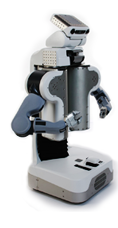
\includegraphics[width=0.25\textwidth]{figs/Introduction/PR2.png}
    \caption{The PR2 robot.}
    \label{fig:PR2}
\end{figure}

\paragraph{Humans and objects detection:} When interacting with humans during manipulation tasks, the robot needs to be able to localize and identify humans and objects. To avoid as much as possible perceptions issues which are not the focus of this thesis, the perception of humans and objects is simplified here. The humans are identified and perceived thanks to a motion capture system. They wear a helmet to get the position and orientation of their heads and a glove to get the position and orientation of their right hands (see Fig.~\ref{fig:Environment}). Concerning the objects, they are identified and localized with tags thanks to the robot cameras in its head.

\begin{figure}[!h]
	\centering
    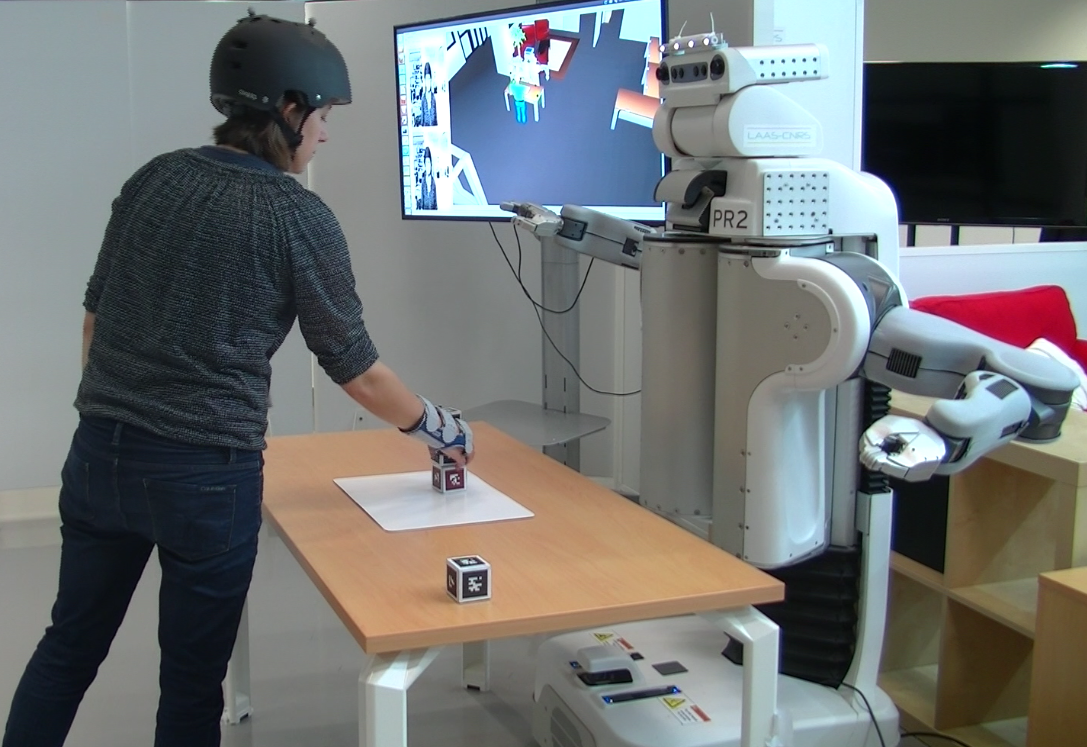
\includegraphics[width=0.7\textwidth]{figs/Introduction/SetUp.png}
    \caption{The PR2 robot interacting with a human to build a stack of cubes. The human is detected thanks to a motion capture system (helmet and glove) and the objects with tags.}
    \label{fig:Environment}
\end{figure}

\newpage
\section*{Publications}
\addcontentsline{toc}{section}{Publications}

The work presented in this thesis has led to several publications. They are listed here bellow (from the most recent to the oldest):
\begin{itemize}
\item \textbf{Devin, S.}, Clodic, A., Alami, R. (2017). About Decisions During Human-Robot Shared Plan Achievement: Who Should Act and How? The Ninth International Conference on Social Robotics. \textit{Submitted}.
\item \textbf{Devin, S.}, Alami, R. (2016). An implemented theory of mind to improve human-robot shared plans execution. In Human-Robot Interaction (HRI), 2016 11th ACM\/IEEE International Conference on (pp. 319-326). IEEE.
\item \textbf{Devin, S}., Milliez, G., Fiore, M., Clodic, A., Alami, R. (2016). Some essential skills and their combination in an architecture for a cognitive and interactive robot. Workshop In Human-Robot Interaction (HRI), 2016 11th ACM\/IEEE International Conference on (pp. 319-326). IEEE.
\item Khamassi, M., Girard, B., Clodic, A., \textbf{Sandra, D.}, Renaudo, E., Pacherie, E., Alami, R., Chatila, R. (2016). Integration of Action, Joint Action and Learning in Robot Cognitive Architectures. Intellectica (ARCo), 2016(65), 169-203.
\item Renaudo, E., \textbf{Devin, S.}, Girard, B., Chatila, R., Alami, R., Khamassi, M., Clodic, A. (2015). Learning to interact with humans using goal-directed and habitual behaviors. In RoMan 2015, Workshop on Learning for Human-Robot Collaboration.
\end{itemize}


\ifdefined\included
\else
\bibliographystyle{StyleThese}
\bibliography{These}
\end{document}
\fi